\section{Integration to the Operating System}
\label{sec:integration}
% Problemas
% EPOS
% Solução: ELUS, Configurabilidade do protocolo, ETP

%This section provides an overview of the \ELUS{}, how its memory consumption is optimized, and how the data dissemination protocol is integrated to the OS infrastructure.

\subsection{\ELUS{} Overview}

%\epos{} (\EPOS{}) is a multi-platform, component-based OS, in which traditional operating system services are implemented through adaptable, platform-independent \emph{System Components}\footnote{\EPOS{} components are encapsulated in C++ classes with well-defined interface and behavior.}~\cite{Frohlich:2001}. Platform-specific support is implemented through \emph{Hardware Mediators}~\cite{Polpeta2004}. Mediators are functionally equivalent to device drivers in UNIX platforms, but do not compose a traditional hardware abstraction layer. Instead, they use platform-independent interfaces to sustain their interface contract between components and hardware. Through the use of static metaprogramming and function inlining, mediator code is \emph{dissolved} into components at compile-time.

%Software reprogramming in \EPOS{} is supported through the \elus{} (\ELUS{})~\cite{Gracioli:2010}.
%\ELUS{} is implemented using the \EPOS{} metaprogrammed framework, around the remote method invocation aspect~\cite{Frohlich:2001}.
Figure~\ref{fig:framework-reconf.pdf} shows the \ELUS{} framework for software reprogramming. The \proxy{} and \agent{} elements create an indirection level between the method invocations from the application and the OS. Thus, the \agent{} is the only member in the system aware of the components' memory location. Consequently, the \agent{} is able to locate and to update the code and data of the system components. Moreover, system components can be marked as reconfigurable or not at compile-time by setting a boolean value in its \textit{Trait} class (\textit{Traits$<$Component$>$::reconfiguration = true}). For those components that are not marked as reconfigurable, no overhead in terms of memory and processing is added in the final system image. The \adapter{} class is responsible for applying the aspects supplied by \scenario{} before and after the real method call~\cite{froehlich:2000}.

%\fig{framework-reconf.pdf}{Modified \EPOS{} framework for supporting software reprogramming.}{scale=.45}
\fig{framework-reconf.pdf}{\ELUS{} framework for software reprogramming.}{scale=.45}

%Method invocations between \proxy{} and \agent{} are done by a function (called \textit{trapAgent}) that has a table (\textsc{Dispatcher}). This table contains all \agent{} method addresses. The \textit{trapAgent} function is responsible for ensuring the quiescent state in an updating, that is, a consistent state in which none of the system threads are calling methods of a component, by using a Semaphore for each component. The \agent{} uses a hash table to keep all system objects and calls the component methods through the virtual method table of an object (\textit{vtable}). When the \agent{} must update a method of a component, it writes the new address into the corresponding \textit{vtable} location.

\subsection{Memory Optimization}

Each component marked as reconfigurable generates an overhead in terms of memory consumption due to the \ELUS{} metaprogrammed framework.
In addition to the real component methods, it is included the code of the framework's methods.
%After the generation of the final system image, the code for each framework method is replicated for each component marked as reconfigurable.
%Moreover, the code for each framework method is replicated for each component marked as reconfigurable.
Moreover, the code for each framework method is replicated for each reconfigurable component.
For example, the method \texttt{update}, responsible for updating the code and data of a component, is replicated for each component. 

By using a template specialization technique it is possible to overcome this limitation.
We observed that several methods from \agent{} and \scenario{} classes can be replaced by template classes that receive a parameter with no type (\textit{void})~\cite{stroustrup:2000}.
%With this simple technique we could reduce the \ELUS{} memory consumption by more than 50\%, without losing performance in terms of method invocation and reconfiguration times, as will be demonstrated in Section~\ref{sec:evaluation}.
With this simple technique we reduce the \ELUS{} memory consumption without losing performance in terms of method invocation and reconfiguration times, as will be shown in Section~\ref{sec:evaluation}.

\subsection{Data Dissemination Protocol Integration}

\ELUS{} receives a reprogramming request for a component through a protocol, called \etp{} (\ETP{}). 
This protocol defines the format of updating messages.
%Figure~\ref{fig:msg_add_en} exemplifies one available message type.
%The control byte defines the message type and amount of fields of that message.
A thread, created during the system's initialization, named \textsc{Reconfigurator}, creates a data dissemination protocol instance and after receiving the new data, starts the reprogramming process.
It is possible to add or remove a method, update the entire component (all methods), update the application, add attributes, and update a specific address. In case of updating/adding attributes values, the data state transfer between the new and old component's attributes is done by the \textit{set} and \textit{get} methods of each attribute.

%\begin{figure}[ht!]
%\centering
%	\subfigure[] {
%	
\includegraphics[scale=0.5]{fig/msg_add_en}
%	\label{fig:etp_add}
%	}
%	\subfigure[] {
%	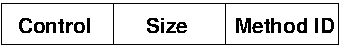
\includegraphics[scale=0.5]{fig/msg_rem_en}
%	\label{fig:etp_rem}
%	} 
%	\subfigure[] {
%	
\includegraphics[scale=0.5]{fig/msg_upd_en}
%	\label{fig:etp_upd}
%	}
%	\subfigure[] {
%	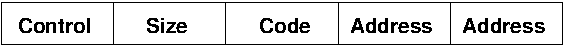
\includegraphics[scale=0.5]{fig/msg_app_en}
%	\label{fig:etp_app}
%	}
%\caption{Reprogramming messages in the \ETP{} format. (a) Adding a method (b) removing a method (c) updating a component (d) updating the application.}
%\label{fig:etp}
%\end{figure}

%\fig{msg_add_en}{Reprogramming message in the \ETP{} format: adding a new method}{scale=.5}

This message structure allows an easy integration of a data dissemination protocol and the OS. The data dissemination protocol mounts messages in the \ETP{} format and calls the \agent{} informing an updating. This simple message structure is not found in the related works, but it is essential to abstract and provide a simple updating process for developers. 
%Figure~\ref{fig:sequence_reprog.pdf} shows the UML sequence diagram for the updating process and the integration between the \ELUS{} and the data dissemination protocol.
Figure~\ref{fig:sequence_reprog.pdf} shows the UML sequence diagram for the updating process.
The \textsc{Reconfigurator} starts the protocol by calling the method \textit{run}.
This method stays blocked until a new version is received by the node.
After receiving the new data, the \textsc{Reconfigurator} creates a message in the \ETP{} format and passes the data to \agent{} (\textit{trapAgent}).
The \agent{} writes the new component code into the appropriate location and updates all tables, if necessary.
 
\fig{sequence_reprog.pdf}{Integration between the data dissemination protocol and ELUS.}{scale=.45}
